\documentclass{beamer}

\usepackage[utf8]{inputenc}
\usepackage[english]{babel}

\usetheme{Berlin}

\title{Pattern Recognition and Machine Learning}
\author{\textbf{Team 5} - Tzanetis Savvas, Zoidis Vasileios}
\date{\today}

\begin{document}
\begin{frame}
    \titlepage
\end{frame}

\section{Part A}
    \begin{frame}{Part A}    
    In this first part of the assignment, we are tasked with quantifying stress levels of video game players based on play patterns
    and the intensity of button presses. Given the stress index $x$, which reflects the frequency and pressure of key presses, we are
    tasked with implementing a \textbf{Maximum Likelihood Estimator} that should correctly predict whether a player is experiencing
    stress, by distinguishing between two classes $\omega_1$ (no stress) and $\omega_2$ (stress).
    \end{frame}

    \begin{frame}{Part A}
    We are also given:
    \begin{itemize}
    \item The \textbf{PDF} function for the indicator $x$ 
    \[
    p(x|\theta) = \frac{1}{\pi(1+(x-\theta)^2)}
    \]
    \item The discriminant function
    \[
    g(x) = \log{P(x|\hat{\theta}_1)} - \log{P(x|\hat{\theta}_2)} + \log{P(\omega_1)} - \log{P(\omega_2)}
    \]
    \end{itemize}
    \end{frame}

    \begin{frame}{Part A1}
    The first requirement for this part of the assignment is to estimate the variables $\hat{\theta_1}$ and $\hat{\theta_2}$.
    In order to achieve this, we need to implement the \textbf{Log Likelihood} function:
    \[
    \log{L(\theta|D) = \sum_{x \in D}\log{p(x|\theta)}}
    \]
    As well as define a range of candidate $\hat{\theta}$ values, which will likely contain the true $\hat{\theta}$. 
    \end{frame}

    \begin{frame}{Part A1}
    This is done because using an approach like the gradient of $\log{L(\theta | D)}$ would be computationally expensive, as
    this function does not have a closed-form expression. The range of $\hat{\theta}$ candidates should be a slightly wider 
    that the range of our data \textbf{[-4.5,  4.1]} to ensure that the optimal value will be included. This range will be 
    \textbf{[-6.0, 6.0]}.
    \end{frame}

    \begin{frame}{Part A1}
    The estimated $\hat{\theta}_1$ and $\hat{\theta}_2$ values, as well as the $\log{p(D_1 | \theta)}$ and $\log{p(D_2 | \theta)}$, are shown in the graph below:
    \begin{figure}
        \centering
        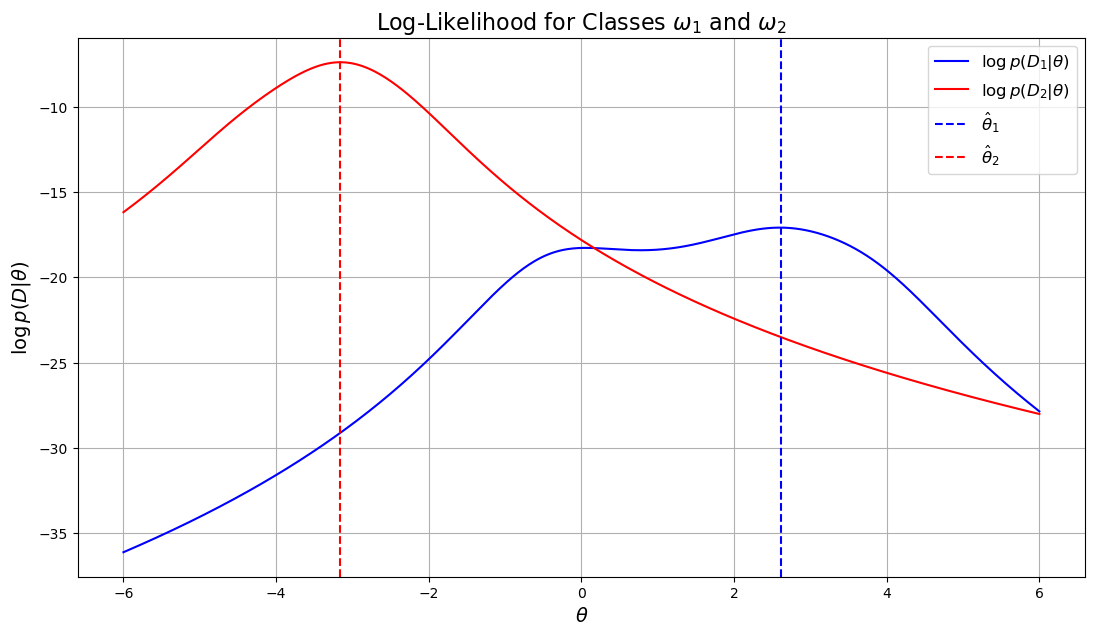
\includegraphics[width=0.75\linewidth]{A1.png}
        \label{Graph A1}
    \end{figure}
    \end{frame}

    \begin{frame}{Part A2}
    Next we need to classify the two datasets $D_1$ and $D_2$, using the discriminant function that was provided in the beginning:
    \[
    g(x) = \log{P(x|\hat{\theta}_1)} - \log{P(x|\hat{\theta}_2)} + \log{P(\omega_1)} - \log{P(\omega_2)}
    \]
    \begin{figure}
        \centering
        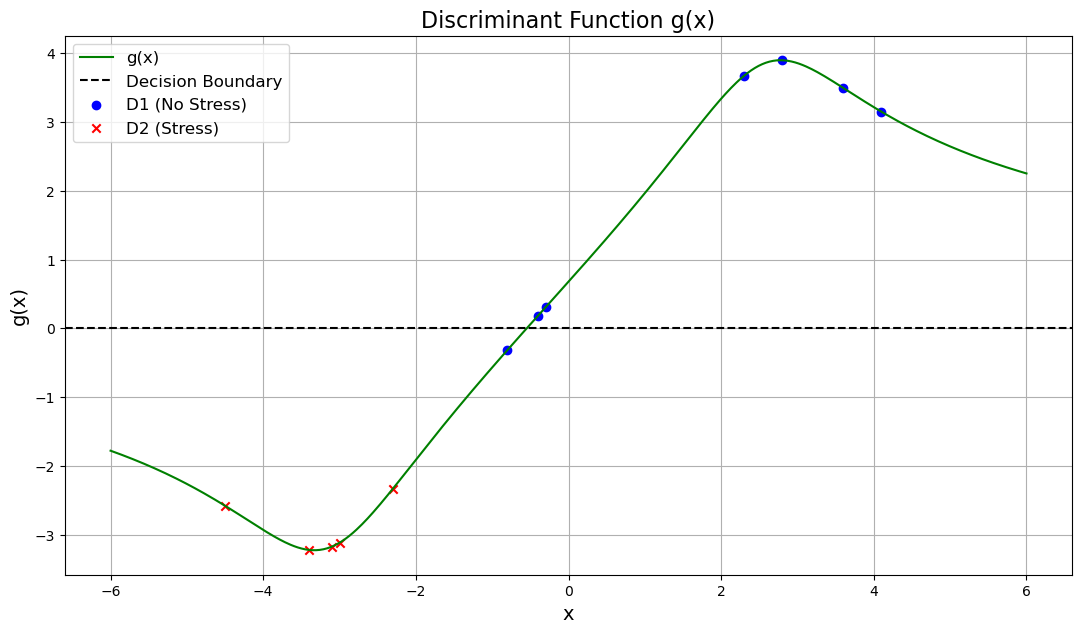
\includegraphics[width=0.75\linewidth]{A2.png}
        \label{Graph A2}
    \end{figure}
    \end{frame}

    \begin{frame}{Part A2}
    In conclusion, with the decision boundary at \textbf{$g(x) = 0$}, meaning that any point in $g(x) < 0$ is classified 
    as \textbf{stress} and any point in $g(x) > 0$ is classified as \textbf{no stress}, we have the following results:
    \begin{itemize}
        \item \textbf{11} out of \textbf{12} values of the $D_1$ dataset are classified correctly.
        \item All of the values of the $D_2$ dataset are classified correctly.
    \end{itemize}
    \end{frame}

\section{Part B}
    \begin{frame}{Part B}    
    In this second part of the assignment, we are again tasked with quantifying the stress level of video game players. This time however, we are asked to use the \textbf{Bayesian estimation method} since we are given the \textbf{Probability Density Function} of $\theta$:
    $$
    p(\theta) = \frac{1}{10\pi \left( 1 + \left(\frac{\theta}{10}\right)^2 \right)}
    $$
    \end{frame}

    \begin{frame}{Part B}
    This means that we are now able to calculate the \textbf{a posteriori probability} of $\theta$, $P(\theta|D)$ like so:
    $$
    P(\theta|D)=\frac{P(\theta|D)p(\theta)}{\int_{-\infty}^{\infty} P(\theta|D)p(\theta) \, d\theta}
    $$
    \end{frame}

    \begin{frame}{Part B1}
    Plotting the \textbf{a posteriori probability} for each dataset \textbf{$P(\theta|D_1)$} and \textbf{$P(\theta|D_2)$} we can observe that:
    \begin{figure}
        \centering
        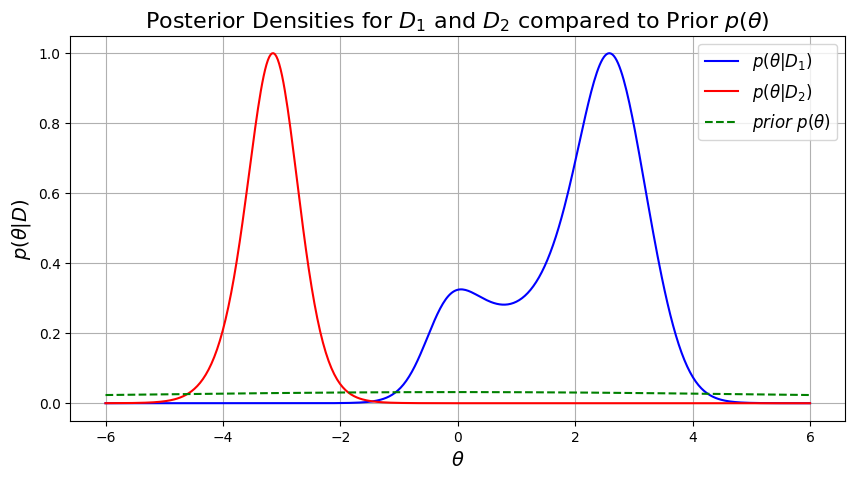
\includegraphics[width=1\linewidth]{B1.png}
        \label{Graph B1}
    \end{figure}
    \end{frame}

    \begin{frame}{Part B1}
    Observations:
    \begin{figure}
        \centering
        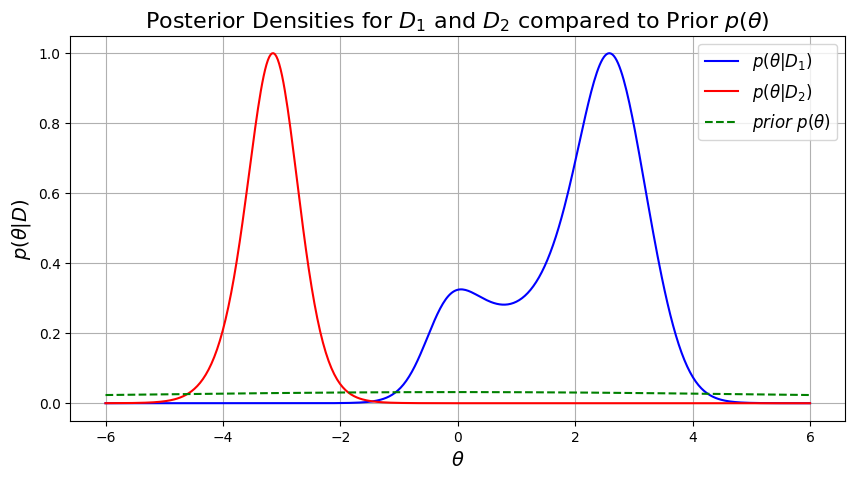
\includegraphics[width=0.75\linewidth]{B1.png}
        \label{Graph B1}
    \end{figure}
    The \textbf{location of the peaks} in the posterior distributions $P(\theta|D_1)$ and $P(\theta|D_2)$ shows the impact of each dataset ($D_1$ and $D_2$).
    \end{frame}

    \begin{frame}{Part B1}
    Observations:
    \begin{figure}
        \centering
        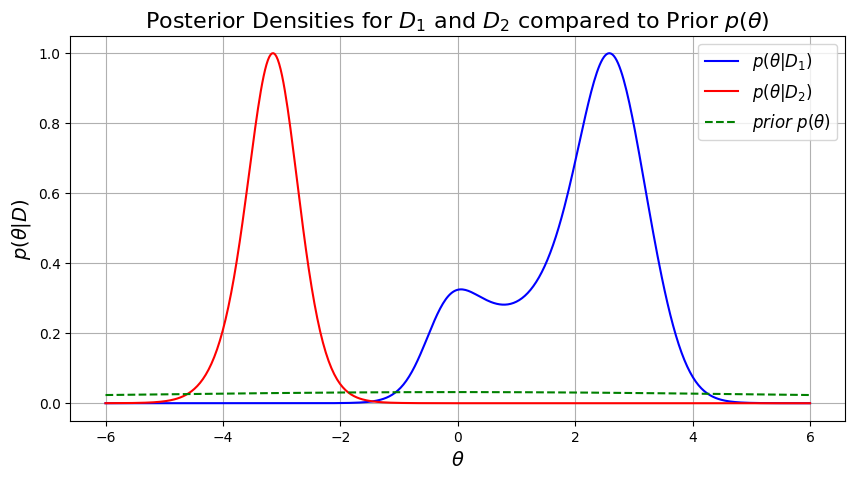
\includegraphics[width=0.75\linewidth]{B1.png}
        \label{Graph B1}
    \end{figure}
    The \textbf{prior} $p(\theta)$ is \textbf{broad} and \textbf{evenly distributed} across the range of $\theta$ values, indicating \textbf{little preference for any particular} $\theta$.
    \end{frame}
    
    \begin{frame}{Part B1}
    Observations:
    \begin{figure}
        \centering
        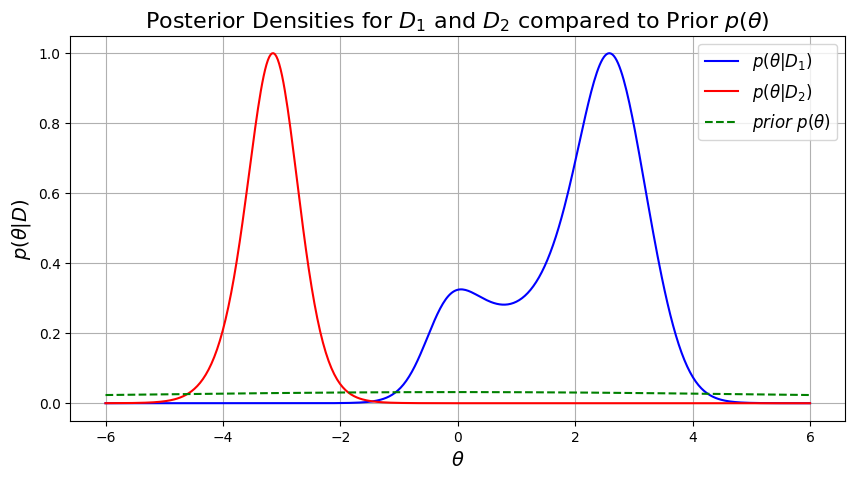
\includegraphics[width=0.75\linewidth]{B1.png}
        \label{Graph B1}
    \end{figure}
    The \textbf{posteriors} are much \textbf{more concentrated} compared to the prior, showing how the data refines the prior belief and provides more accurate estimates of $p(\theta)$.
    \end{frame}

    \begin{frame}{Part B2}
    At this point, we are tasked to classify the two datasets using \textbf{this discriminant function}:
    $$
    h(x) = \log{P(x|D_1)} - \log{P(x|D_2)} + \log{P(\omega_1)} - \log{P(\omega_2)}
    $$
    In order to implement this, we declare this \textbf{posterior predictive distribution} ${P(x|D)}$ as:
    $$
    P(x|D)={\int P(x|\theta)P(\theta|D) \, d\theta}
    $$
    \end{frame}

    \begin{frame}{Part B2}
    Now, we can visualize $h(x)$:
    \begin{figure}
        \centering
        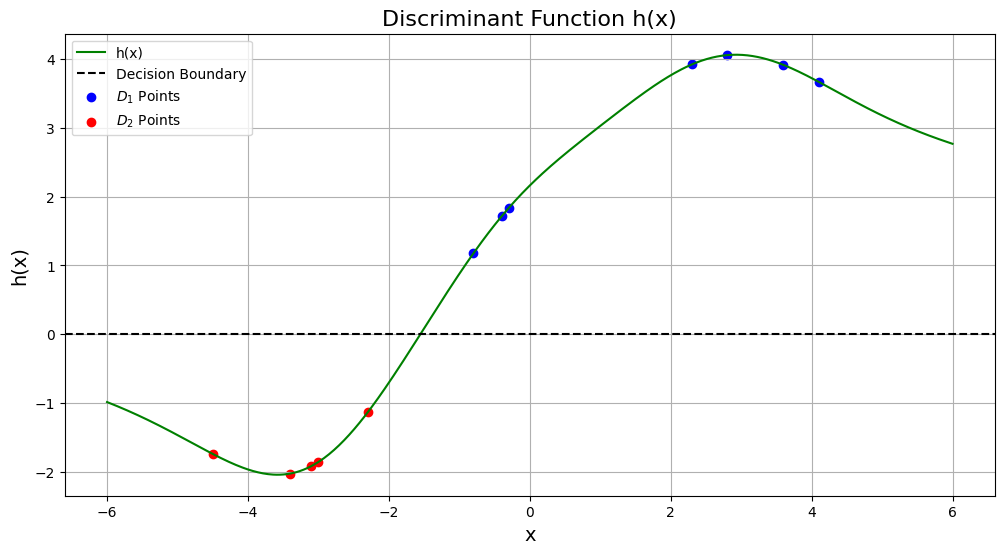
\includegraphics[width=1\linewidth]{B2.png}
        \label{Graph B1}
    \end{figure}
    \end{frame}

    \begin{frame}{Part B2}
    Observations:
    \begin{figure}
        \centering
        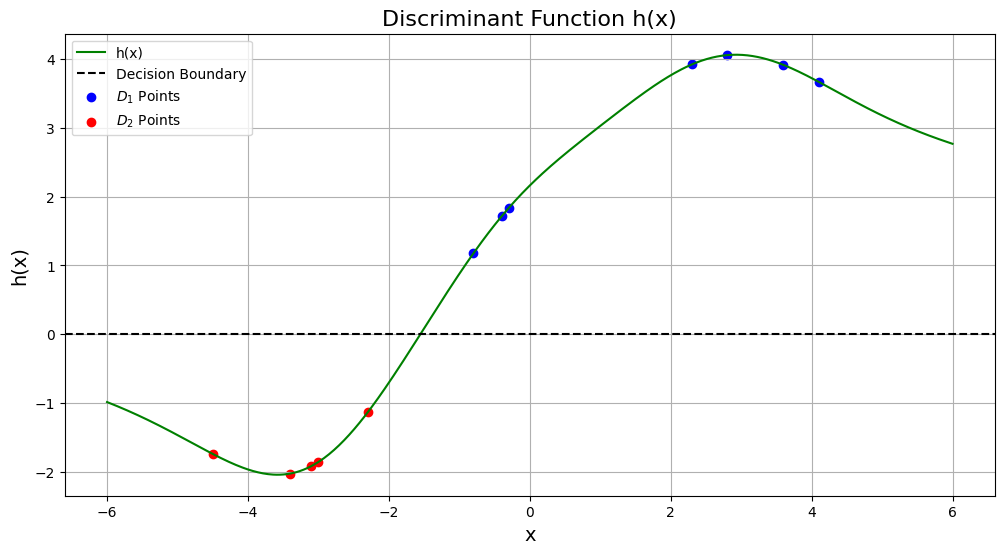
\includegraphics[width=0.75\linewidth]{B2.png}
        \label{Graph C1}
    \end{figure}
    The \textbf{decision boundary} is at $h(x)=0$, and \textbf{correctly}, all the points of $D_1$ are classified \textbf{above} the decision boundary and all the points of $D_2$ are classified \textbf{below} the decision boundary.
    \end{frame}

    \begin{frame}{Part B2}
    \fontsize{12}{13.5}{\textbf{Bayesian Estimation} vs \textbf{Maximum Likelihood} method:}
    \hfill\break\hfill\break
    In this specific example, the Bayesian Parameter Estimation method is preferred over the Maximum Likelihood method, since it classifies the data with \textbf{100\%} accuracy, as opposed to the Maximum Likelihood approach \textbf{91.7\%}. Most likely, this discrepancy is due to the fact that in part B we have prior knowledge about the \textbf{Probability Density Function} $\theta$.
    \end{frame}

\section{Part C}
    \begin{frame}{Part C}
        In this part, we are tasked to train a \textbf{Decision Tree Classifier} on three specific \textbf{Iris species} (Iris setosa, Iris versicolor, and Iris virginica) using the sepal length and width of each plant.
        \hfill\break\hfill\break
        Meaning, we have \textbf{two features} and \textbf{three classes}.
    \end{frame}

    \begin{frame}{Part C1}
        First, we \textbf{load} the Iris dataset and \textbf{isolate} only the first two features. Subsequently, we \textbf{split} the dataset into a training and a testing set \textbf{(50\%:50\%)} and \textbf{define} random state in order to ensure reproducibility.
        \hfill\break\hfill\break
        Then, we \textbf{train} the Decision Tree Classifier and \textbf{evaluate} its performance for \textbf{various} depths.
    \end{frame}

    \begin{frame}{Part C1}
        We aim to find the \textbf{best depth} of Decision Tree Classifier in regard to \textbf{accuracy}.
        \hfill\break\hfill\break
        After testing for depth in a range of up to 10 to avoid overfitting, we conclude that the optimal depth is \textbf{3} with \textbf{78.67\%} accuracy.
    \end{frame}

    \begin{frame}{Part C1}
        Therefore, we use the \textbf{best model} (with a depth of 3) to classify our data:
        \begin{figure}
        \centering
        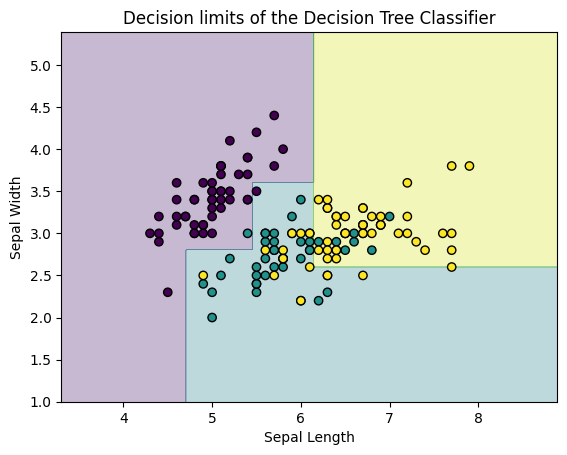
\includegraphics[width=0.65\linewidth]{C1.png}
        \label{Graph C1}
    \end{figure}
    \end{frame}

    \begin{frame}{Part C2}
       Now, we are tasked to \textbf{create} 100 new training sets from 50\% of the original training set each time and \textbf{train a Random Forest classifier} with 100 trees using the \textbf{Bootstrap} technique.
    \end{frame}

    \begin{frame}{Part C2}
       First, we will need to create the \textbf{100 samples} for the Bootstrap technique ($\gamma$ = 50\%).
       \hfill\break\hfill\break
       Then, we can \textbf{train} the Random Forest Classifier and \textbf{evaluate} its performance for \textbf{various} depths. Similar to before, we are testing for depth in a range of up to 10 to avoid overfitting.
    \end{frame}

    \begin{frame}{Part C2}
        We conclude that the optimal depth is \textbf{2} with \textbf{82.67\%} accuracy:
        \begin{figure}
        \centering
        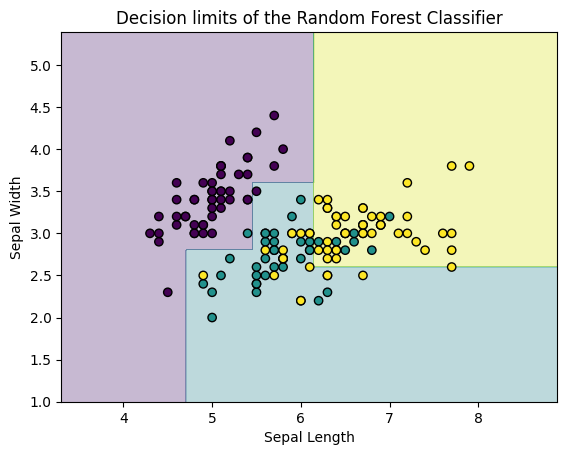
\includegraphics[width=0.65\linewidth]{C2.png}
        \label{Graph C2}
    \end{figure}
    \end{frame}

    \begin{frame}{Part C2}
    \fontsize{12}{13.5}{\textbf{Random Forest} vs \textbf{Decision Tree} classifier:}
    \hfill\break\hfill\break
    We remark that the \textbf{Random Forest } slightly outperforms the \textbf{Decision Tree} classifier. More specifically, we observe a \textbf{5\% improvement} in terms of accuracy. This discrepancy is due to the nature of Decision Trees, which create \textbf{rough decision boundaries} (hard splits) and often result in \textbf{overfitting} to the training data. In contrast, Random Forests produce \textbf{smoother decision boundaries} and \textbf{less overfitting} because they \textbf{average} the predictions from multiple trees. This has the effect of mitigating the overfitting typically seen in a single Decision Tree and enabling \textbf{better generalization}.
    \end{frame}

    \begin{frame}{Part C2}
    \fontsize{12}{13.5}{How does the \textbf{percentage $\gamma$} affect the performance of the algorithm?}
    \hfill\break\hfill\break
    From the analysis we did, we observe that:
    \begin{itemize}
        \item for \textbf{lower $\gamma$ values} (0.1, 0.2, 0.3) the accuracy varies between \textbf{0.80} and \textbf{0.81}, showing slight improvements as $\gamma$ increases.
        \item For \textbf{higher values} (0.4 and above), accuracy \textbf{stabilizes} around \textbf{0.83},  suggesting diminishing returns in performance improvement with increasing $\gamma$.
    \end{itemize}
    \end{frame}

    \begin{frame}{Part C2}
       In general, \textbf{smaller $\gamma$ values} result in \textbf{higher bias} because each bootstrap set includes less information about the entire dataset.
       \hfill\break\hfill\break
       Conversely, \textbf{larger $\gamma$ values} reduce diversity among the bootstrap sets, which can \textbf{limit the ensemble's ability to mitigate variance} effectively.
       \hfill\break\hfill\break
       In summary, increasing $\gamma$ \textbf{up to 0.4} enhances the algorithm's performance, but \textbf{further increases have no significant impact} on accuracy.
    \end{frame}

\section{Part D}
    \begin{frame}{Part D}
    In the final part of the assignment, we are tasked with training a classification model of our choice using a provided
    dataset  \textbf{(datasetTV.csv)} and later make predictions on a test dataset \textbf{(datasetTest.csv)}. The TV dataset
    consists of:
    \begin{itemize}
        \item \textbf{8743} samples.
        \item \textbf{224} features per sample.
    \end{itemize}
    While the test dataset has no labels as it is only meant to test the trained model on and has:
    \begin{itemize}
        \item \textbf{6955} samples.
        \item \textbf{224} features per sample as well.
    \end{itemize}
    \end{frame}

    \begin{frame}{Part D - Data Scaling}
    Before fitting a model to our datasets, we must first \textbf{scale} the data of both the training and test sets.
    This is an essential step as this ensures that all features contribute equally to the model's decision-making process,
    as features with larger scales won't be able to dominate the learning process.
    \end{frame}

    \begin{frame}{Part D}
    In order to choose a suitable model, we tested several different classifiers and their prediction accuracy 
    using \textbf{5-Fold cross validation}. More specifically we tested:
    \begin{itemize}
        \item A \textbf{k-NN} classifier with a score of \textbf{0.81}
        \item A \textbf{Secure Vector Machine} classifier with a score of \textbf{0.83}
        \item A \textbf{Random Forest} classifier with a score of \textbf{0.80}
        \item A \textbf{Decision Tree} classifier with a score of \textbf{0.72}
    \end{itemize}
    \end{frame}

    \begin{frame}{Part D - Validation Score}
    \textbf{5-Fold cross validation} is a technique commonly used for evaluating the performance of a decision model,
    as it is great at assessing its performance on unseen data since:
    \begin{itemize}
        \item The dataset is divided randomly in \textbf{5} equal sized sub-sets (folds), where in each of the 5 iterations,
        4 out of the 5 folds are used for training the model and the other is used as a test set.
        \item After all 5 iterations are complete, we calculate the mean accuracy across all iterations.
    \end{itemize}
    \end{frame}

    \begin{frame}{Part D - Validation Score}
    \begin{figure}
        \centering
        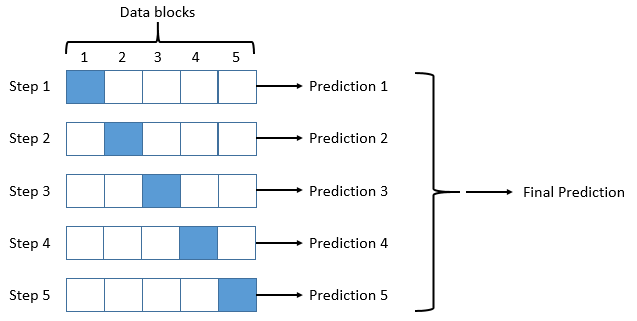
\includegraphics[width=0.75\linewidth]{D1.png}
        \label{Graph A2}
    \end{figure}
    \end{frame}

    \begin{frame}{Part D}
    The classification model we ended up choosing was a \textbf{Support Vector Machine (SVM)} classifier as it had the best 5-Fold
    cross validation accuracy among all the other classification models we tested. The \textbf{SVM} classifier was the best option,
    as it is able to handle high-dimensional spaces like the one in our dataset effectively, while also being less prone to
    overfitting. Scaling the data like previously mentioned, is especially important as it ensures that the optimization
    algorithm moves at a consistent rate for all features.
    \end{frame}

    \begin{frame}{Part D - Parameter Tuning}
    After deciding on a model, we need to tune its parameters in order to maximize its prediction accuracy. 
    In order to do this performed a \textbf{Grid Search} as well as a \textbf{Random Search}, since calculating
    the accuracy of all possible combinations of parameters is very computationally expensive.
    \end{frame}

    \begin{frame}{Part D - Parameter Tuning}
    Beginning with a \textbf{Grid Search}, the parameters that were tested, as well as their possible values are seen below:
    \begin{itemize}
        \item Kernel: \textbf{rbf}, \textbf{linear}.
        \item C: \textbf{1, 10, 100}.
        \item Gamma value $\gamma$: \textbf{scale, auto}.
    \end{itemize}
    \end{frame}

    \begin{frame}{Part D - Parameter Tuning}
    \textbf{Grid Search} on its own has some disadvantages. Since every possible combination of parameters is being tested,
    testing a large number of possible parameters can get very computationally expensive since we are also testing combinations
    of parameters that are unlikely to yield acceptable results.
    \end{frame}

    \begin{frame}{Part D - Parameter Tuning}
    This is why we also used the \textbf{Random Search} technique, which allows us to define a range of possible values and 
    test them by randomly sampling values for each parameter. While this method can be efficient, it may not always find the
    'optimal' result because it doesn't exhaustively explore the parameter space. For this reason, it is used in conjunction with 
    \textbf{Grid Search}, which systematically tests all possible combinations of parameters.
    \end{frame}

    \begin{frame}{Part D - Parameter Tuning}
    Combining the results of both techniques, the optimal values that we used for our classification model where:
    \begin{itemize}
        \item Kernel: \textbf{rbf}.
        \item C: \textbf{4}.
        \item: Gamma value $\gamma$: \textbf{scale}.
    \end{itemize}
    \end{frame}

    \begin{frame}{Part D - Final Results}
    Finally, our \textbf{Support Vector Machine} classification model with specified parameters, yields acceptable results, with
    \textbf{5-Fold cross validation} scores of: [0.864, 0.858, 0.851, 0.850, 0.839], and a mean score of \textbf{0.85}.
    The relatively small variance in scores across each iteration of the cross-validation assures us that there is no
    overfitting in our trained model.
    \end{frame}
    
\end{document}
